\pagebreak
\section{Overall Description}
\subsection{Product perspective}
% il prodotto e' self-contained. (???)

The software-to-be is going to be made of several parts: two front-end applications for the customers, a different one for the taxi drivers and an API for developers. 

Concerning the customer interface, it will be pretty similar to other related apps (for example, Uber or MyTaxi), since it will supply similar functions. It will primarly let them reserve or request a taxi.

As for the taxi drivers, a simpler interface will be given, since only one functionality will be developed (accepting a request for a ride).
 
\subsubsection{User interfaces}
The application will have two client interfaces, a web app and a mobile app. For simplicity's sake, here are presented the mobile interfaces only.

\pagebreak
\paragraph{Home}
The home app page. Clicking on "Call a taxi" opens the "Request a taxi" screen.
\begin{center}
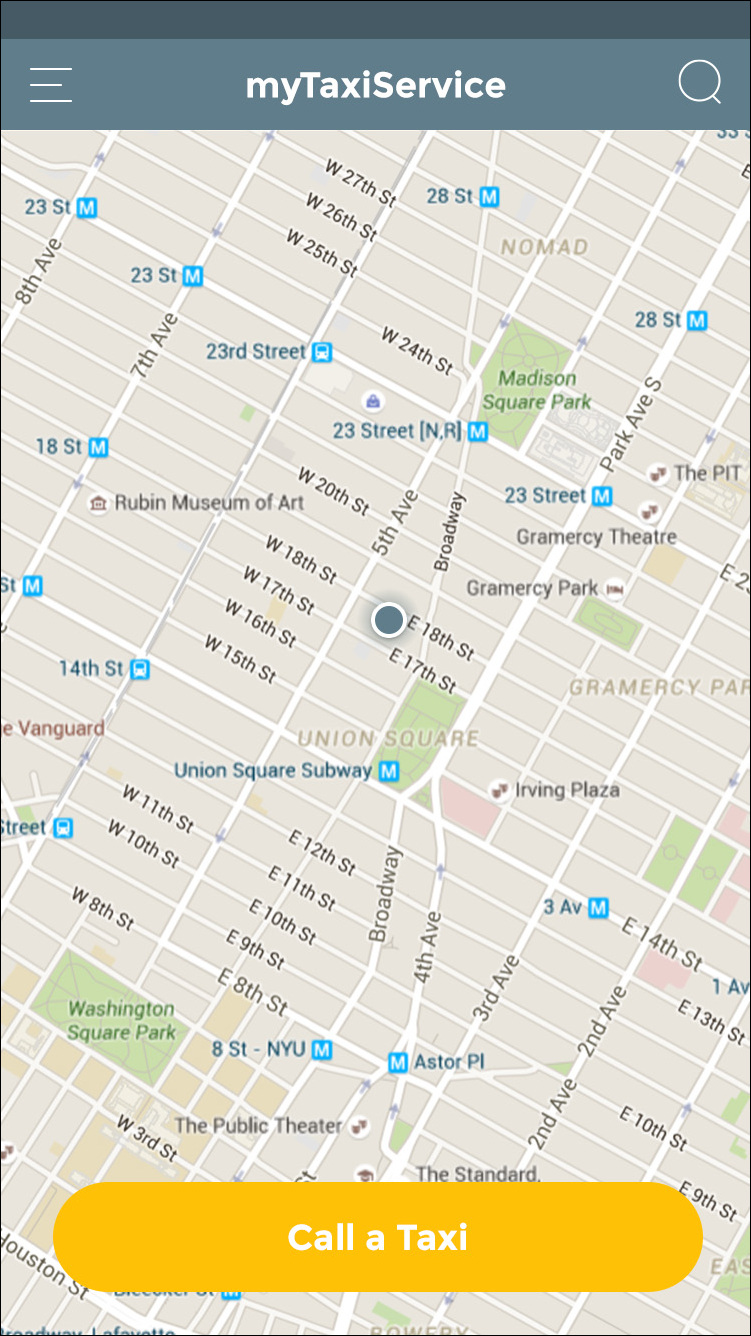
\includegraphics[scale=0.5]{mockup_home.jpg}
\end{center}

\pagebreak
\paragraph{Log in}
The login screen for a customer.
\begin{center}
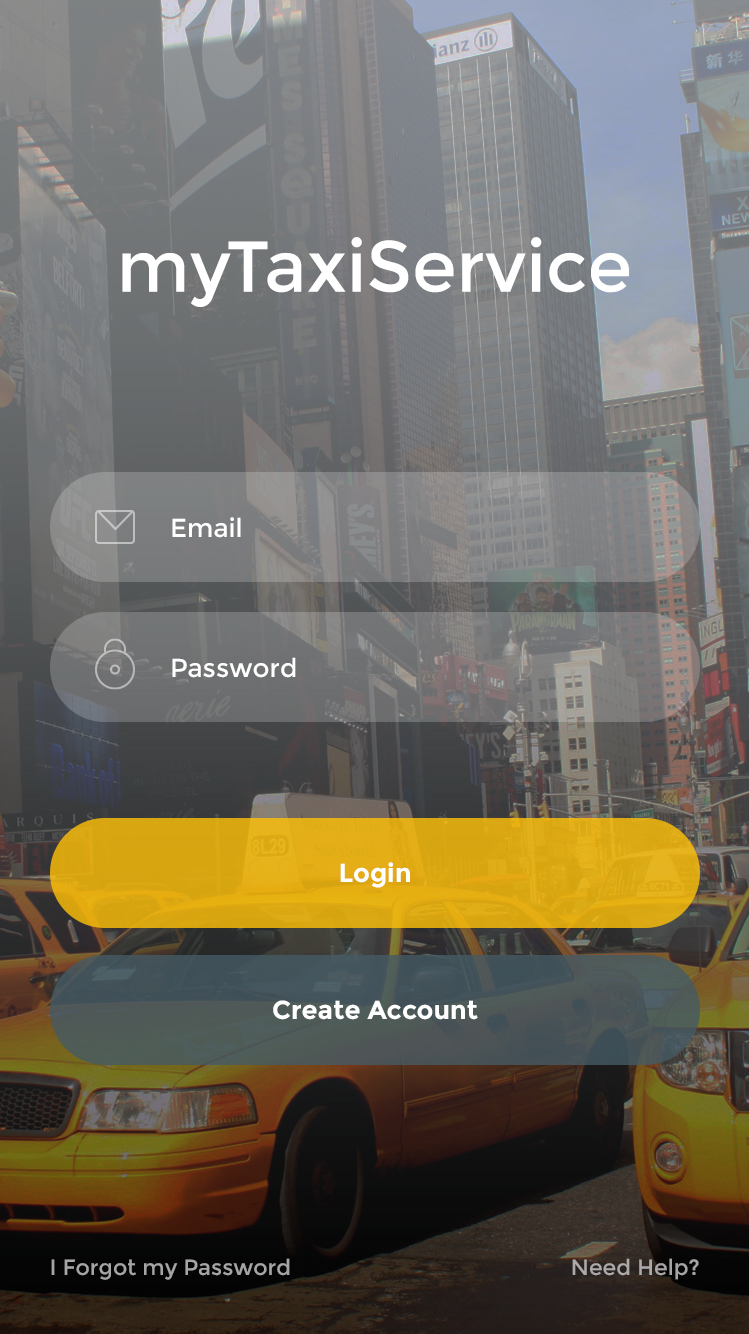
\includegraphics[scale=0.5]{mockup_login.jpg}
\end{center}

\pagebreak
\paragraph{Sign up}
The registration page for a guest willing to become a customer.
\begin{center}
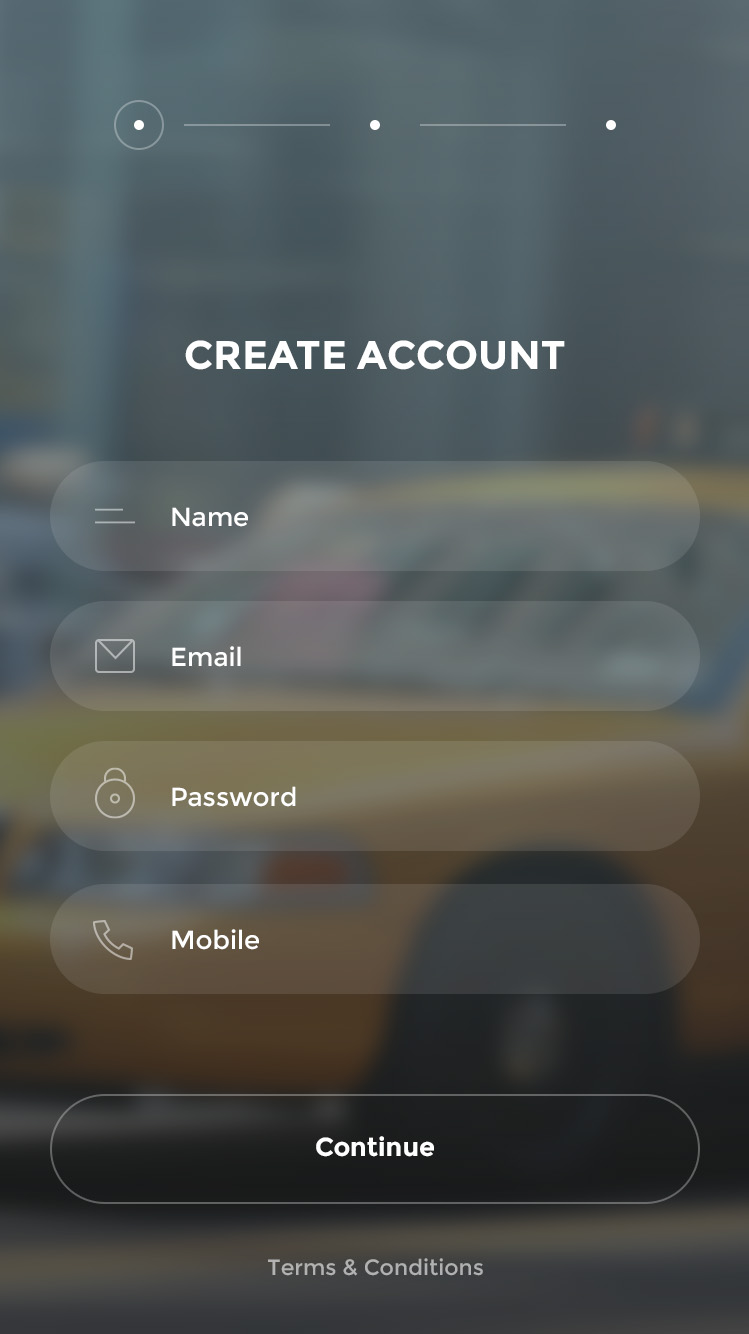
\includegraphics[scale=0.5]{mockup_signup.jpg}
\end{center}

\pagebreak
\paragraph{Reserve a taxi}
Here is the page where a customer can reserve a taxi for a specified day. Starting point, destination and time are mandatory information. The mockup also illustrates the "Sharing" option enabled. The "Request a taxi" functionality uses a stripped-down version of this window (no sharing option, only current day available)
\begin{center}
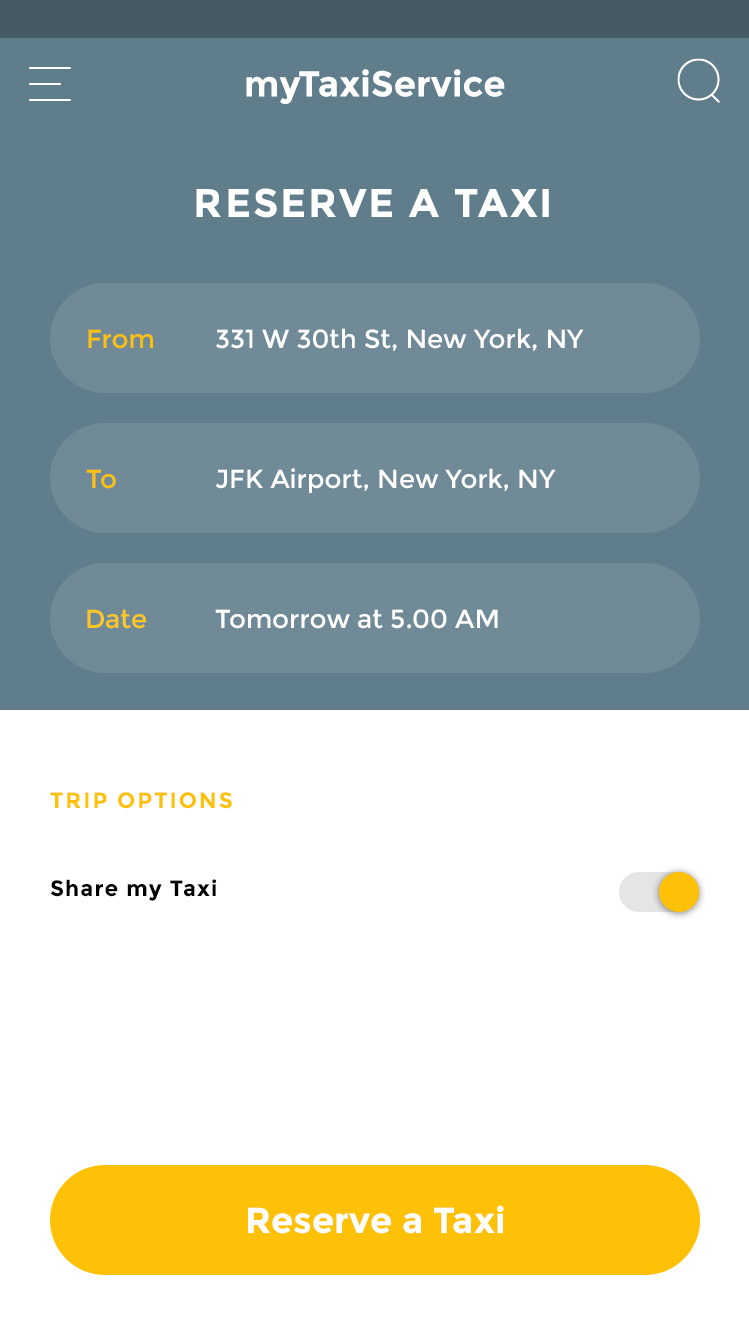
\includegraphics[scale=0.5]{mockup_reserve.jpg}
\end{center}

\pagebreak
\paragraph{Confirmation screen}
After requesting or reserving a taxi, the service shows you a confirmation screen, 
\begin{center}
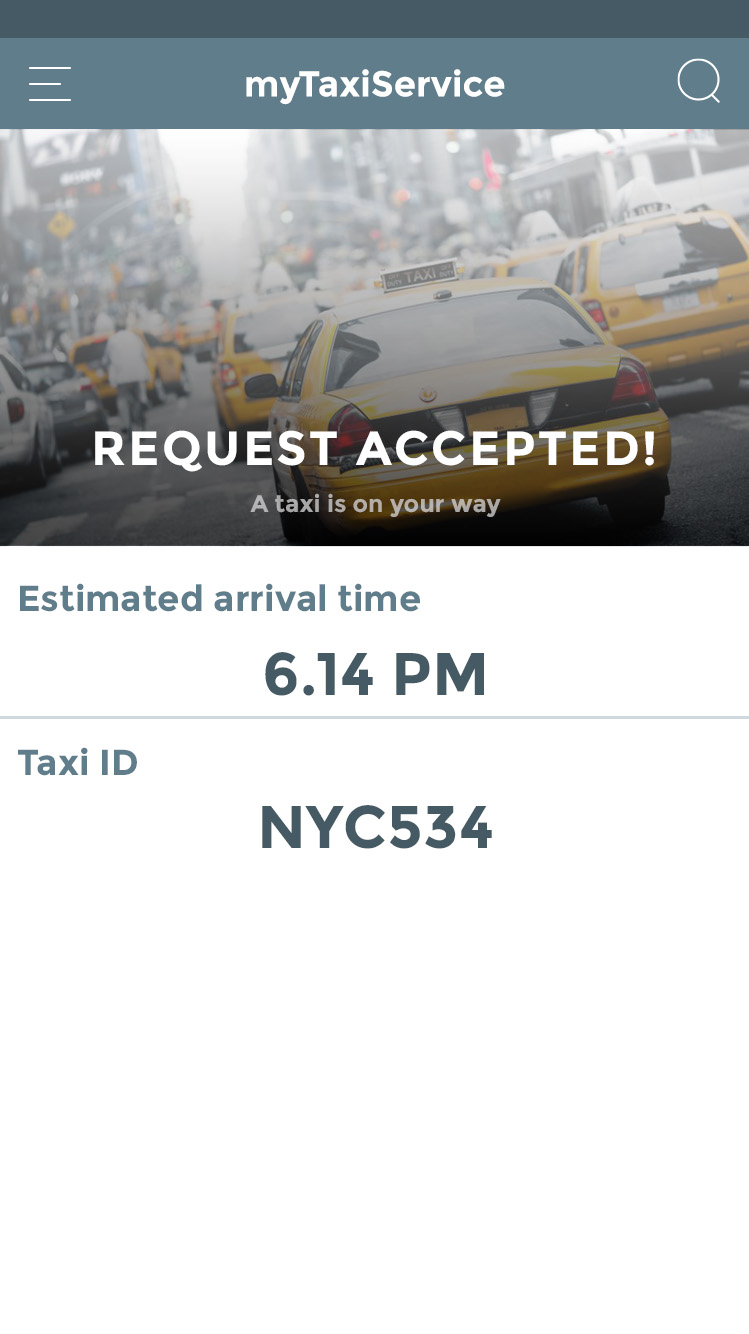
\includegraphics[scale=0.5]{mockup_confirm.jpg}
\end{center}

\pagebreak
\paragraph{Notification to a taxi driver}
This shows how the notification appears on a taxi driver's smartphone. No web app interfaces available for this functionality.
\begin{center}
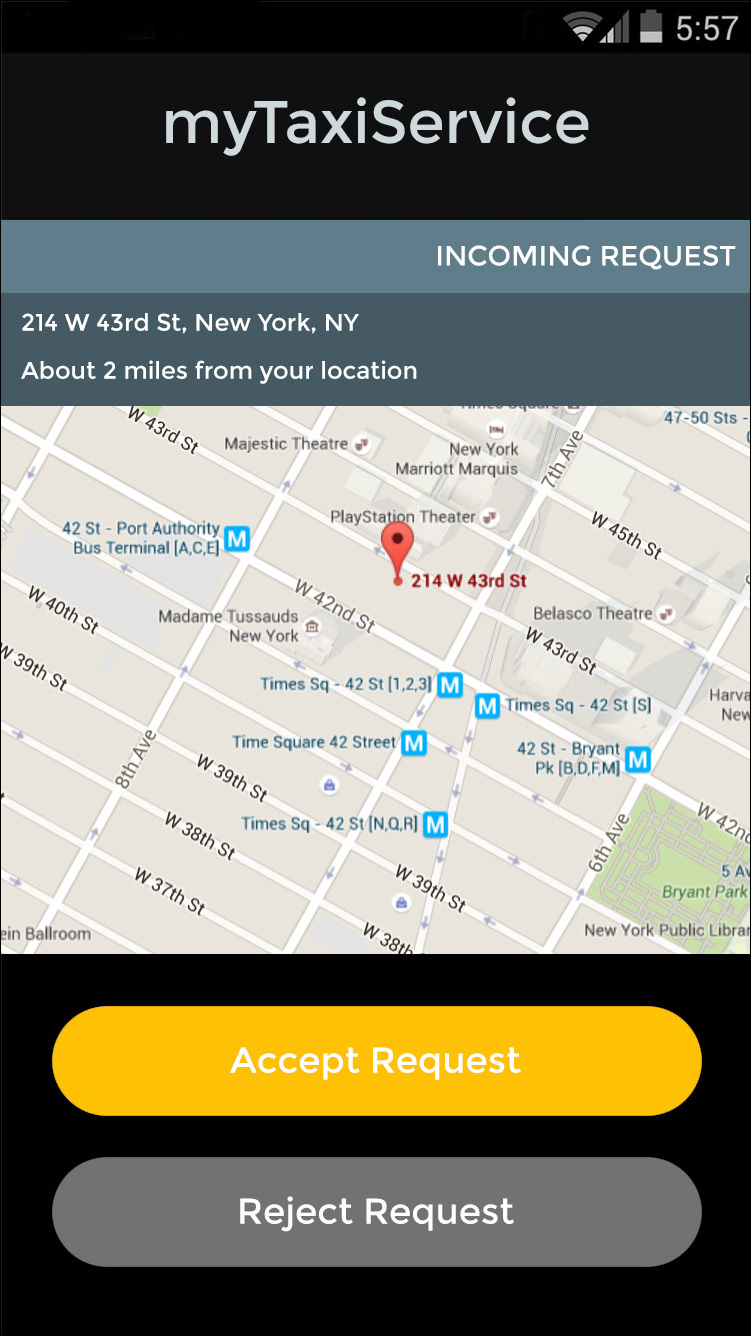
\includegraphics[scale=0.5]{mockup_call.jpg}
\end{center}

\pagebreak
\subsubsection{Hardware interfaces}
In order to correctly use myTaxiService, a GPS system is required in order to track all vehicles and distribute them fairly in each zone. In addition to this, some vehicles have a point-of-sale terminal (POS), which is expressely indicated in the system; this way, if a user chooses to pay with a credit card, only POS-enabled cars are used to grant the service.

\subsubsection{Software interfaces}
\begin{itemize}
\item Back-end
\begin{itemize}
	\item DBMS:
	\begin{itemize}
		\item Name: MySQL
		\item Version: 5.7
		\item Source: http://www.mysql.it/
	\end{itemize}
	
	\item Programming language:
	\begin{itemize}
		\item Name: PHP
		\item Version: 5.6.7
		\item Source: http://www.php.net/
	\end{itemize}
	
	\item Operating System:
	\begin{itemize}
		\item Name: Linux Debian
		\item Version: 8.2
		\item Source: https://www.debian.org/
	\end{itemize}	
	
	\item Map API:
	\begin{itemize}
		\item Name: Google Maps
		\item Source: https://developers.google.com/maps/
	\end{itemize}	
\end{itemize}

\item Front-end
\begin{itemize}
\item Operating System (for both customers and taxi drivers):
	\begin{itemize}
		\item Android
		\item iOS
		\item Blackberry
	\end{itemize}
\end{itemize}
\end{itemize}

\pagebreak
\subsection{Constraints}

\subsubsection{Interfaces to other applications}
% layer con servizio taxi gia' esistente

\subsection{Assumptions and Dependecies}
Here is a list of domain assumptions and dependecies the writers of this document assume to hold in the real world:
\begin{itemize}
\item There already is a geolocalization system for each taxi, based on the GPS information
\item Each request is sent to one taxi at a time
\item Each taxi driver actually serves a request if he accepted it
\item A taxi driver is available only when in his own vehicle 
\item If a customer reserves or requests a taxi, he will use it

\end{itemize}
